\documentclass[a4paper 10pt]{article}
\usepackage[english,polish]{babel}
\usepackage[MeX]{polski}
\usepackage[utf8]{inputenc}
\usepackage[T1]{fontenc}
\usepackage[letterpaper, portrait, margin=1in]{geometry}
\usepackage{graphicx}
\usepackage{listings}
\usepackage{subfigure}
\usepackage{dashrule}
\usepackage{listings}
\usepackage{float}
\usepackage{amsmath}
\usepackage{listings}
\usepackage{multirow}
\usepackage{amsmath}
\usepackage{xcolor}
\usepackage{listings}
\usepackage{hyperref}
\hypersetup{ hidelinks = true, } 
\lstset{
    frame=single,
    breaklines=true,
    postbreak=\raisebox{0ex}[0ex][0ex]{\ensuremath{\color{red}\hookrightarrow\space}}
}


\renewcommand{\rmdefault}{ptm}
  
\frenchspacing

% Used to add additional dot in enumerations
\usepackage{titlesec}
\titlelabel{\thetitle.\quad}
\title{\textbf{Techniki Optymalizacji} \\
Laboratorium nr 2 \\
Sprawozdanie}
\author{Paulina Sadowska, Rafał Araszkiewicz}
\begin{document}
\maketitle

\section{Wprowadzenie}
Celem ćwiczenia było poprawienie wyników otrzymanych przez algorytmy Nearest Neighbour i Greedy Cycle poprzez zastosowanie lokalnego przeszukiwania. w wersji stromej Otrzymane wyniki porówanano z otrzymanymi po wyznaczeniu losowej ścieżki i nastepnie zastosowaniu lokalnego przeszukiwania.
\section{Local search}
\label{Local search}
W algorytmie tym trasa budowana jest w taki sposób, że dla wygenerowanego wcześniej rozwiązania szukamy takiej pary wierzchołków lub pary krawędzi które po zamianie pozwolą na otrzymanie krótszej ścieżki. Następnie wykonujemy zamianę, która pozwoli na uzyskanie największego zysku. Kroki te należy powtarzać tak długo, jak mozliwe jest znalezienie takiej pary wierzchołków lub krawędzi których zamiana skróci scieżkę.
\subsection{Implementacja w pseudokodzie}
\begin{lstlisting}[frame=single]
dopoki zmiana trasy zmniejsza jej koszt

	dla kazdego z punktow na sciezce
		staryKoszt = koszt przejscia do punktu + koszt przejscia z punktu do nastepnego
		dla kazdego punktu spoza sciezki
			nowyKoszt = koszt przejscia do nowego punktu + koszt przejscia z nowego punktu do nastepnego
			jezeli nowyKoszt < minKoszt oraz nowyKoszt < staryKoszt
				minKoszt = nowyKoszt 
				
	dla kazdej pary punktow na sciezce
		dla kazdej kolejnej pary punktow na sciezce
			stayKoszt = koszt przejscia miedzy para nr 1 + koszt przejscia miedzy para nr 2
			nowyKoszt = koszt przejscia miedzy pierwszymi punktami z kazdej z par + koszt przejscia miedzy drugimi punktami z kazdej z par
			jezeli nowyKoszt < minKoszt oraz nowyKoszt < koszt
				minKoszt = nowyKoszt			
	
	jezeli zysk z zamiany wierzcholkow jest wiekszy niz z zamiany krawedzi
		zamien punkt sciezki na ten dajacy lepszy zysk
	jezeli zmiana krawedzi przyniesie zysk	
		zamien  krawedzie miejscami
	w przeciwnym razie
		opusc petle
	
koniec

\end{lstlisting}
\label{Local search code}
\section{Najlepsze ścieżki}
\subsection{Nearest Neighbour + Local Search}
%\begin{figure} [H]
%\centering
%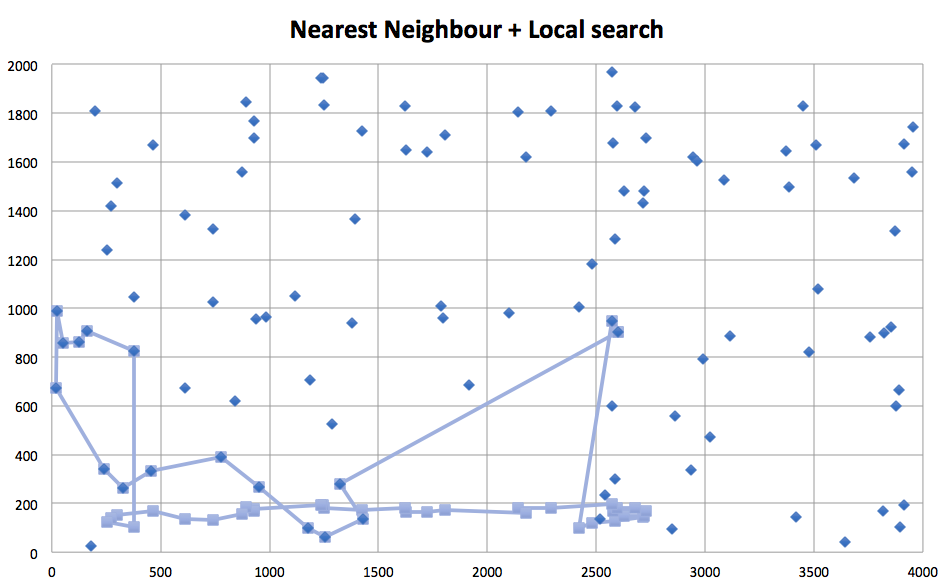
\includegraphics[angle=0,width = 1\textwidth, height=!]{images/NN.png}
%\caption{Najlepsza trasa - Nearest Neighbour}
%\label{Rys. NN}
%\end{figure}

\subsection{Greedy Cycle + Local Search}

\subsection{Nearest Neighbour Grasp + Local Search}

\subsection{Greedy Cycle Grasp + Local Search}

\section{Otrzymane wyniki}

\begin{table}[H]
\centering
\caption{Otrzymane wyniki}
\label{my-label}
\begin{tabular}{|l|l|l|l|l|l|}
\hline
             & NN + LS & GC + LS & NN Grasp + LS & GC Grasp + LS & Random + LS \\ \hline
min cost     &         &         &               &               &             \\ \hline
average cost &         &         &               &               &             \\ \hline
max cost     &         &         &               &               &             \\ \hline
best path    &         &         &               &               &             \\ \hline
best time    &         &         &               &               &             \\ \hline
average time &         &         &               &               &             \\ \hline
worst time   &         &         &               &               &             \\ \hline
\end{tabular}
\end{table}


\end{document}